\documentclass[12pt]{book}

\usepackage{amsmath}
\usepackage{hyperref}
\usepackage{color}
\usepackage{enumerate}
\usepackage{fancyhdr}
\setlength{\headheight}{30pt}


\setlength{\oddsidemargin}{0cm}
\setlength{\evensidemargin}{0cm}
\setlength{\textwidth}{6.5in}
\setlength{\topmargin}{-2.2cm}
\setlength{\textheight}{9.3in}
 \pagestyle{plain}
\pagestyle{fancyplain}
\fancyhf{}
\lhead{ \fancyplain{}{ABC Player} }
\rhead{ \fancyplain{}{Andrei Ivanov, Olga Shestopalova, Zeke Schmois} }
\rfoot{ \fancyplain{}{\thepage} }

\renewcommand{\arraystretch}{1.5}	
\newcommand{\Ri}{\ \Rightarrow\ }
\newcommand{\Le}{\ \Leftarrow\ }
\newcommand{\Lr}{\ \Leftrightarrow\ }
\newcommand{\ds}{\displaystyle}
\newcommand{\ts}{\textstyle}
\newcommand{\sst}{\scriptstyle}
\newcommand{\sss}{\scriptscriptstyle}
\newcommand{\q}{\quad}
\newcommand{\ap}{\alpha}
\newcommand{\ii}{\^{\i}n }
\newcommand{\si}{\c{s}i }
\newcommand{\oaf}{oricare ar fi }
\newcommand{\nn}{\mathbb{N}}
\newcommand{\ns}{\mathbb{N}^{*}}
\newcommand{\rr}{\mathbb{R}}
\newcommand{\rs}{\mathbb{R}^{*}}
\newcommand{\cc}{\mathbb{C}}
\newcommand{\zz}{\mathbb{Z}}
\newcommand{\zs}{\mathbb{Z}^{*}}
\newcommand{\qq}{\mathbb{Q}}
\newcommand{\qs}{\mathbb{Q}^{*}}
\newcommand{\g}{\mathbb{G}}
\newcommand{\di}{\displaystyle}
\newcommand{\ai}{astfel \^{\i}nc\^{a}t }
\newcommand{\la}{\lambda}
\newcommand{\s}{\sigma}
\newcommand{\ri}{\ \rightarrow\ }
\newcommand{\gr}{^{\circ}}
\usepackage{graphicx}


\begin{document}
%%%%%%%%%%%%%%%%%%%%%%%%%%%%%%%%%%%%
%%%%%%%%%%%%%%%%%%%%%%%%%%%%%%%%%%%%
%%%%%%%%%%%%%%%%%%%%%%%%%%%%%%%%%%%%
%%%%%%%%%%%%%-------1------%%%%%%%%%%%%%%%%%
%%%%%%%%%%%%%%%%%%%%%%%%%%%%%%%%%%%%
%%%%%%%%%%%%%%%%%%%%%%%%%%%%%%%%%%%%
%%%%%%%%%%%%%%%%%%%%%%%%%%%%%%%%%%%%
%%%%%%%%%%%%%%%%%%%%%%%%%%%%%%%%%%%%
\phantom{xxx}
\bigskip
\centerline{{\large \bf ABC Parser Project: Design Description }}
\bigskip\bigskip

\noindent {\textbf{Overview:}}

We represent an ABC parser for music files as a series of well-structured interfaces. When an ABC Music file is selected from the menu, it will be read and converted into a string, which will then be passed to the lexer to create tokens, which are then fed to the parser to walk the tree and create {\tt Music} objects, which then provide the necessary information to create and play the MIDI file created.

\bigskip
\noindent {\textbf{Revision Summary:}}
\bigskip

The lexer was changed to read duplet, triplet, and quadruplet parenthesis and digit as one token (so no quintuplets and up are allowed). The parser was changed to include a line rule that groups measures with lyrics to make adding lyrics to particular measures easier. It also was changed to include duplet, triplet, and quadruplet rules, also to make it easier to find and modify the notes associated with those.\\

Why we completely redid the g4: The grammar for the subset that was provided didn’t seem to work how we wanted, it would confuse text and notes, and generally fail in all aspects. Thus, we completely redid it, keeping on the basic structure of abc tune being made up of abc header and abc music. 
We made each header its own token because it was mainly the content inside that was confusing the lexer and parser, and it would be easy to strip off the newlines and initial letter followed by a colon. Lyrics are also lexed and parsed as the entire line, and then passed off to another grammar, because the symbols in music confused the rest of our grammar, and it seemed appropriate since they were a completely different part of the music (here we focused more on the notes) to make our design more modular.
Furthermore, we decided to lex the notes together with their modifiers, because our smallest object was a note, not a modifier, and it was fairly simple to get the information from the modifiers when we knew what note they were associated with. 
We made a line and measure rule because we needed the lyrics to be associated with a line, and we needed notes associated with a measure (ultimately, we needed lyrics to be associated with a measure, but there was no way to do this directly). 
The way we have it now, the rules play directly into the objects we create in the Listener (Pitch, Rest, Chord, Measure, Lyric etc). \\

A big improvement on the parsing of lyrics was made to the project. In an effort to create modularity, the main grammar parser will feed a stream of lyrics directly into the lyrics parser which works independently. This second parser is robust, simple to read, and ready for change. It proved time and time again to be perfectly ``black-boxed'' in the sense that it never failed due to dependency issues and was always easy to fix internally. Details are provided at the bottom of this document.\\

Main was modified to include a pop up window to select the song to play. This user interface (UI) is designed to help the user play particular songs. They are divided in three categories which is done for clarity. 
The file implements a simple JFrame UI which makes it easier for the user to play any valid .abc file. The instructions are simple:

\begin{itemize}
\item Copy the .abc file into any of the three *\_abc folders (otherSongs, sample, or songs).
\item Run main and click on the song (it gets uploaded automatically)
\end{itemize}

\noindent {\textbf{Abstract Data Types}}

\bigskip
 {\tt Music} is an interface that will represent our ADT. All {\tt Music} objects are immutable. 

 {\tt MusicPart} is an interface that extends {\tt Music} and represents any music part. This could be a {tt MusicPiece}, a {\tt Measure}, or a {\tt Voice} . 

 {\tt MusicSymbol} is another interface that extends {\tt Music} and represents  either a {\tt Pitch}, a {\tt Rest} or a {\tt Chord}.

The representation of our ADT is as follows:


\bigskip
\noindent  Music=MusicPart+MusicSymbol
\medskip

      \noindent MusicPart=MusicPiece($voices$: List$<$Voice$>$, $signature$: Signature) +
 \\ \phantom{MusicPart=}Voice($measures$: List$<$Measure$>$) +
 \\ \phantom{MusicPart=}Measure($notes$: List$<$MusicSymbol$>$, $lyrics$: Lyric)

\medskip

      \noindent MusicSymbol=Chord($notes$: List$<$MusicSymbol$>$, $length$: Fraction) +
 \\ \phantom{MusicSymbol=}Pitch($length$: Fraction, $value$: char, $octave$: int, $accidental$: int) +
 \\ \phantom{MusicSymbol=}Rest($length$: Fraction)

\medskip

\newpage


\noindent{Following is the diagram which underlies our abstract datatypes.} 

\centerline{ 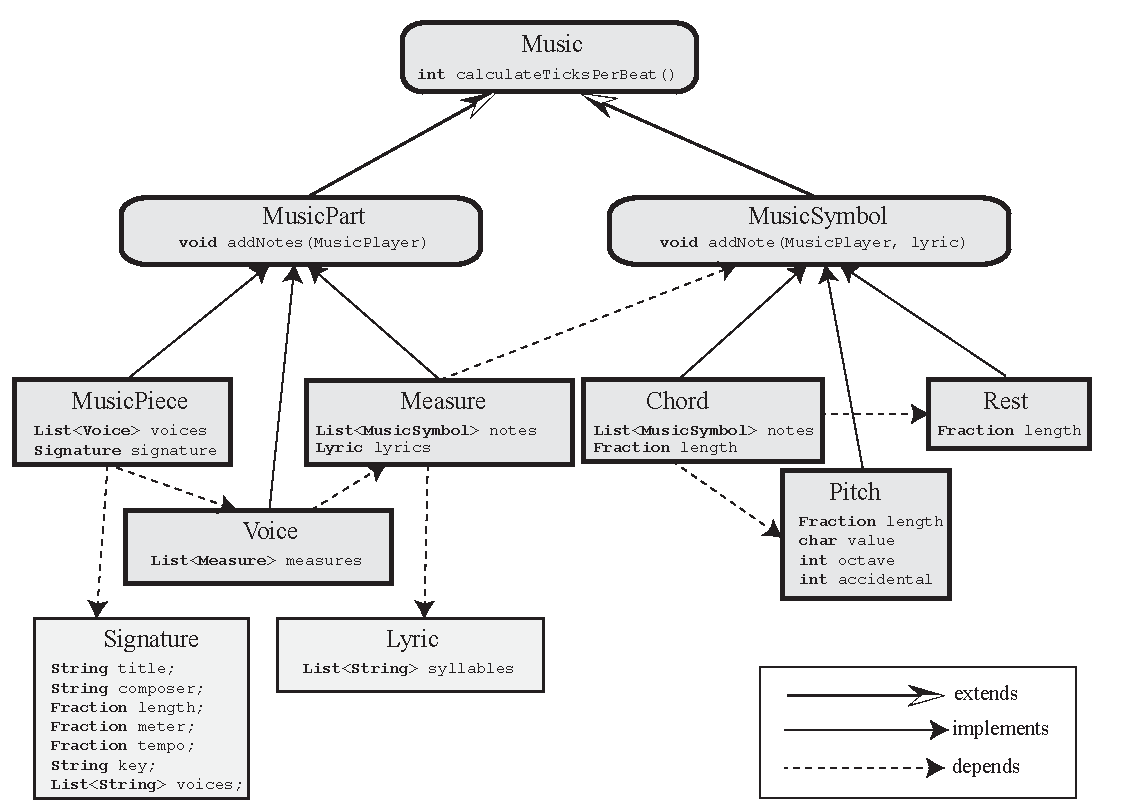
\includegraphics{Music_revised.pdf}}

\noindent\makebox[\linewidth]{\rule{\textwidth}{0.4pt}}

All {\tt Music} objects have equals, toString, and hashCode methods  that work recursively and individually different from each class extending {\tt Music}. Read their documentation for full specs (interface package).
{\tt Music} interface also defines the following method

\begin{itemize} 

\item { \tt calculateTicksPerBeat} is an auxiliar method needed to determine the number of ticks per beat for the player such that any notelength can be represented as an integer number of ticks. The method is called recursively.
\end{itemize}


\noindent\makebox[\linewidth]{\rule{\textwidth}{0.4pt}}

\smallskip
\noindent {\tt MusicPart} interface  defines the method method
\begin{itemize} 
\item { \tt addNotes} which takes an instance of  {\tt MusicPlayer} (described later) and adds to it all notes and lyrics found in the current {\tt MusicPart}  . It is called recursively.
\end{itemize}

\noindent and is implemented by the following classes:
\begin{itemize} 
\item { \tt MusicPiece} represents a final piece of music.   It has a {\tt signature} attribute which contains all the header information and {\tt List<Voice> voices} attribute which represents a list of different voices contained in this piece.
\item {\tt Voice}  represents a single voice in a piece of music. It has a {\tt List<Measure> measures } attribute which represents the sequence of measures the voice is made of.
\item {\tt Measure}  represents a single measure in a voice. It has a {\tt List<MusicSymbol>notes } attribute which represents the sequence of notes contained in the measure and a  {\tt List<Lyric> lyrics } attribute that represents the lyrics that accompain the measure.
\end{itemize}
\noindent\makebox[\linewidth]{\rule{\textwidth}{0.4pt}}

\smallskip
\noindent {\tt MusicSymbol} is  interface defines the  method
\begin{itemize} 
\item { \tt addNote} which takes an instance of  {\tt MusicPlayer} and a lyric corresponding to the current symbol and modifies the player by adding notes and lyric to it. 
\end{itemize}
\noindent and is implemented by classes:
\begin{itemize} 
\item { \tt Pitch} represents a single pitch. Its attribute {\tt length} is represented by a fraction  of the length of the default note. The attribute {\tt value} is a pitch A,B,C,...,G from the middle octave,  {\tt octave} represents the offset from the middle octave and  {\tt accidental} is 1 for sharp and -2 for flat. Using these conviniences,  a {\tt Pitch} from out ADT can be easily converted to the {\tt Pitch} object described in the {\tt sound} package.
\item { \tt Rest} represents a single rest and has an attribute {\tt length}  represented by a fraction of the length of the default note. 
\item {\tt Chord} represents a chord of several pitches and stores them in the {\tt List<Pitch>} attribute.
\end{itemize}

\noindent\makebox[\linewidth]{\rule{\textwidth}{0.4pt}}

These three basic music symbols let us implement any "musical expression" defined in the 6.005 subset. Any other structures like tuplets, triplets, repeats, etc. are converted to these basic music symbols during the ParseTree walk.  

We also use an immutable class {\tt Signature} inside MusicPiece that has all header information stored in its attributes and a mutable class {\tt Lyric} which represents a list of lyrics used for each measure.


\noindent\makebox[\linewidth]{\rule{\textwidth}{0.4pt}}

\medskip
Another important class is a mutable {\tt MusicPlayer} which has three attributes 
\begin{itemize} 
\item { \tt player} that represents an instance of the {\tt SequencePlayer}. It collects the notes and lyrics of the song.
\item { \tt ticksPerBeat} which represents the number of ticks per beat in the {\tt player}
\item { \tt currentTick} which represents the current tick inside the player. It is used when the notes and lyrics are added consecutively to the player by the method {\tt addNote} to keep track of the position  where the notes need to be inserted. {\tt addNote} method increments it according to the length of the note.
\end{itemize}
It has the following methods:
\begin{itemize} 
\item { \tt addNote (int note,Faction length)} that takes a converted Midi note and inserts it in the {\tt player} at the {\tt currentTick} position, moving the pointer to the tick the note finishes at.
\item { \tt addLyric (String Lyric)} that takes a syllable and adds it to the {\tt LyricListener} at the {\tt currentTicks} position.
\item { \tt addTime (Fraction length)} increases the {\tt currentTick} by the length of the note.
\item { \tt resetTime() } resets the {\tt currentTicks} to 0. This is used when starting a new voice.
\item { \tt play() } plays the notes and lyrics added by calling {\tt SequencePlayer}'s {\tt play} method. 
\end{itemize}

\bigskip

\noindent { \large \bf Parsing }

\bigskip

\begin{itemize}
\item {\bf Lexer}: The lexer is designed such that all of the header lines (ie. title, composer, etc) are each lexed as one token, as are all lyric and comment lines. Notes are lexed together with their modifiers (accidentals, octaves, duration) as one token. Duplet, triplet, and quadruplet parenthesis and digits are lexed as a single token (apart from their notes). Chord brackets are lexed separately from their notes. Pipes, repeats, and end of measure symbols are lexed as their own tokens. All whitespace except for newlines (/n/r) is skipped.

\item {\bf Parser}: The parser has rules for the whole musical piece, which is then broken into the header rules and the actual musical body rules. Each header line has its own rule, with title, number and key being mandatory. The musical body consists of either lines, voices, and/or comments. 

Lines are measures followed by a newline, optionally followed by a lyric. Measures are note elements optionally surrounded by repeats or pipes, but must end with either a repeat, an end of measure symbol, or a newline. 

A note element is a note, rest, chord, duplet, triplet, or quadruplet. Duplets, triplets, and quadruplets are the particular header token followed by 2, 3, or 4 notes or chords, respectively. A chord is a number of notes or rests enclosed in square brackets. Note, rest, and lyric have their own rules as well, which are just their respective lexer tokens.

\item {\bf Errors}: Errors in parsing and lexing result in an exception being thrown. (reportErrorsAsExceptions is invoked on both parser and lexer).

\item {\bf Listener}: While parsing the tree, we care about these events: exit note, exit rest, exit duplet, exit triplet, exit quadruplet, exit chord, enter measure, exit measure, enter line, exit line, exit lyric, enter voice, exit header, exit tune. Several stacks are present at once, for each kind of object.

When exiting the tune, voices and signature will be added to a MusicPiece object, which is then added to the stack.

When exiting a header, the information is extracted from the context, and defaults are added if necessary. A default voice is set if none are provided. The current voice is kept track of.

When entering a voice, the current voice is switched.

When entering a line, a new list of repeated ranges is created.

When exiting a line, lyrics are matched with their notes in their measure, and padded as necessary. Measure objects are created and added to the stack. If the measure index matches an index in the repeated range, that measure is added again (to the top of the stack). 

When entering and exiting a measure, repeats/n-th repeat/end of line symbols are searched for and the repeated range list is updated accordingly.

When exiting a lyric, the chunk of text will be sent to another lexer and parser, which will return a list of lists of syllables, which will be pushed to the stack.

When exiting a chord, the number of notes or rests inside is determined, then they are popped, and then added to a Chord object, which is then added to the stack (this object represents a list of notes, since they all start at the same time).

When exiting a duplet, triplet, or quadruplet, notes inside are popped, and their duration is modified accordingly, and the new notes are inserted back into stack.

When exiting a note or rest, we extract the needed information from the context and add a Pitch or Rest object to the stack. 


\end{itemize}

\bigskip

\noindent {\large \bf Parsing Lyrics}

\bigskip

\noindent{\textbf {General idea}}
The lyrics parsing is designed to be simple and flexible and at the same time robust and capable of parsing everything deemed a good input. 

\begin{itemize}
\item {\bf Lexer}: We start at the bottom token, LINESPACE. New line tokens are skipped because we have no special action to take when these are encountered. WHITESPACE follows and would normally also be skipped but because of the special WHITESPACE HYPHEN token, we must keep it in (this is explained with more detail in the parser rules). PIPEs are also unique tokens as they are used to separate measures. Then we have all the different symbols used to create different kind of syllables. Most importantly to note is that EXTENDERS and STARS can be one or more of the same while HYPHENs, DOUBHYPHENs, and UNION\_OPERs are composed of single characters. Finally is the WORD token which creates the most complex form of lyric possible, and is composed of all allowed, non-special characters in a lyric.

\item {\bf Parser}:
These rules define the structures used by the parser:
A well constructed lyric will be parsed as follows
\begin{itemize} 
\item lyric:
\begin{itemize}
\item can have multiple measures and any amount of trailing whitespace at the end
\end{itemize}
\item measure:
\begin{itemize}
\item can be an entire lyric if no PIPEs are found
\item can be empty or a cluster (the first word in the cluster determines the first token)
\item if it begins with a PIPE, it may have WHITESPACE*
\item if it ends with a PIPE, optional WHITESPACE* may be used to separate the last syllable
\end{itemize}
\item syllable:
\begin{itemize} 
\item can ONLY start with a WORD or a STARS
\item single syllable and single STARS can be considered a full cluster
\item no combination of WORD and STARS are allowed in the same syllable
\item WHITESPACE* is allowed at the end of every syllable
\item if starting with a WORD it must be followed by:
\begin{itemize}
\item a HYPHEN and\/or EXTENDERS
\item a WHITESPACE and HYPHEN and\/or EXTENDERS
\item a DOUBHYPHEN
\item a UNION\_OPER
\item EXTENDERS
\end{itemize}
\end{itemize}
\end{itemize}

\item Anything outside of these rules will be considered an incorrectly inputed
lyric and will throw an exception\/fail silently with an unexpected outcome

\item {\bf Errors}: Errors in parsing and lexing result in an exception being thrown. (reportErrorsAsExceptions is invoked on both parser and lexer).

\item {\bf Listener}: The lyrics listener is very simple as well. The lyrics object is composed of an ArrayList of ArrayLists of Strings, where each String is a ``syllable''. So, when entering a new Measure, we add an empty ArrayList to the main ArrayList. The only other event is exiting a Syllable. In this case, we consider every valid input and do a second ``parsing'' accordingly. This is actually the pretty-print that we implement for our frontend. It converts things like two-word syllables joined by ``~'' into two words joined by whitespaces.

The end product is an ArrayList<ArrayList<String>>, not null, and processed enough to use a literal toString() method to print to the user's console.
\end{itemize}
\bigskip
\noindent {\large \bf Tests}

\begin{itemize}
\item LexerTest:  Tests the Lexer, ensures tokens are what they should be. Tests headers, headers and body, comments, and all kinds of notes (chords, repeats, tuplets, octaves, accidentals).
 
Testing strategy: Test first the simple cases, then increasingly more complicated and more prone to parsing error cases. Make sure all tokens are correctly lexed and behave the way they should even with whitespace and newlines. Notes should be lexed along with their modifiers. Header lines and comments should be lexed as their own tokens. Tuplet (2, (3, (4 and chord brackets are to be lexed as their own tokens, separate from the notes. Test all modifiers (' ,, \textasciicircum \textasciicircum\textasciicircum \_ \_\_ and durations)!

\item ParserTest: Tests the Parser, ensures that it returns the right objects. Tests basic and extended headers, single and multiple measures and voices, comments, and all kinds of notes (chords, notes with repeats, tuplets, notes with different octaves, notes with accidentals).
 
Testing strategy: Test first the simple cases, then increasingly more complicated and more prone to parsing error cases. Make sure all objects consist of the right objects/components and in the right order. Test all the modifiers (, ,, ' \textasciicircum \textasciicircum\textasciicircum \_ \_\_), all symbols (|]), all repeats (|: :| [1 [2), and all kinds of strange lyrics (* - \\- ~ - -- \_). Make sure accidentals carry over from within the measure and the key (and neutrals stop this).

\item MusicPartTest:  This is the test suite for equals(), toString(), and hashCode() for the classes in the MusicPart interface (other methods are in the no\_didit tests).

Testing strategy: test each method and make sure it is true to its spec for every valid type of input. equals() must return true on equal objects, and false on unequal objects. toString() must provide the appropriate string representation of the object. hashCode() must return a hashcode that is the same for equal objects.
Partition on complexity and modifiers, make sure things that Measures can have 1 or any number of MusicSymbols, Voices can have 1 or any number of measures, and MusicPieces can have 1 and any number of Voices. Also, make sure duration shows up correctly (ie. 1/1 should be nothing, 1/2 should be /2). Test the different modifiers of notes (' , ,, \textasciicircum \textasciicircum\textasciicircum \_ \_\_)

\item MusicSymbolTest:  This is the test suite for equals(), toString(), and hashCode() for the classes in the MusicSymbol interface. The addNote(main) method is tested in MusicPlayerTest.java as its main role is to modify the main.
Moreover, we test the particular methods of the classes that implement the interface: Pitch: multiplyLength(), getLength(), Chord: multiplyLength().

Testing strategy: test each method and make sure it is true to its spec for every valid type of input. equals() must return true on equal objects, and false on unequal objects. toString() must provide the appropriate string representation of the object. hashCode() must return a hashcode that is the same for equal objects.
For Pitch, make sure everything works correctly regardless of how many modifiers there are (, ,, \textasciicircum \textasciicircum\textasciicircum \_ \_\_ and duration), and same for Rest (it only has duration). For Chord, partition on the number of MusicSymbols it has. Also, make sure duration shows up correctly (ie. 1/1 should be nothing, 1/2 should be /2).

\item SignatureTest:  This is the test suite for Signature's equals(), toString(), and hashCode().

Testing strategy: test each method and make sure it is true to its spec for every valid type of input. equals() must return true on equal objects, and false on unequal objects. toString() must provide the appropriate string representation of the object. hashCode() must return a hashcode that is the same for equal objects.
Partition on the number of voices the signature has (1 or more), and how fractions are represented in meter, tempo, and length (ie. how is 4/4 simplified, since usually it would appear as an empty string, but that is inappropriate here).

\item LyricTest: This is the test suite for Lyric's equals(), toString(), hashCode(), and getSyllable().

Testing strategy: test each method and make sure it is true to its spec for every valid type of input. equals() must return true on equal objects, and false on unequal objects. toString() must provide the appropriate string representation of the object. hashCode() must return a hashcode that is the same for equal objects.
Partition on the number of syllables the Lyric has (0 or more) and make sure symbols and whitespace function normally. For getSyllable(), partition on where the syllable is (beginning, middle, end), and size of the array (0 and more elements).

\end{itemize}






\newpage


\end{document}
  
